\documentclass[11pt]{article}
\usepackage{geometry}                
\geometry{letterpaper}                   

\usepackage{graphicx}
\usepackage{amssymb}
\usepackage{epstopdf}
%\usepackage{natbib}
\usepackage{amssymb, amsmath}
\usepackage{hyperref}
\DeclareGraphicsRule{.tif}{png}{.png}{`convert #1 `dirname #1`/`basename #1 .tif`.png}

%\title{Title}
%\author{Name 1, Name 2}
%\date{date} 

\begin{document}



\thispagestyle{empty}

\begin{center}
\includegraphics[width=5cm]{ETHlogo.eps}

\bigskip


\bigskip


\bigskip


\LARGE{ 	Lecture with Computer Exercises:\\ }
\LARGE{ Modelling and Simulating Social Systems with MATLAB\\}

\bigskip

\bigskip

\small{Project Report}\\

\bigskip

\bigskip

\bigskip

\bigskip


\begin{tabular}{|c|}
\hline
\\
\textbf{\LARGE{Evacuation Bottleneck}}\\
\textbf{\LARGE{A look onto the evacuation of a cruise ship}}\\
\\
\hline
\end{tabular}
\bigskip

\bigskip

\bigskip

\LARGE{Benedek Vartok \& Johannes Weinbuch}



\bigskip

\bigskip

\bigskip

\bigskip

\bigskip

\bigskip

\bigskip

\bigskip

Zurich\\
December 2009\\

\end{center}



\newpage

%%%%%%%%%%%%%%%%%%%%%%%%%%%%%%%%%%%%%%%%%%%%%%%%%

\newpage
\section*{Agreement for free-download}
\bigskip


\bigskip


\large We hereby agree to make our source code for this project freely available for download from the web pages of the SOMS chair. Furthermore, we assure that all source code is written by ourselves and is not violating any copyright restrictions.

\begin{center}

\bigskip


\bigskip


\begin{tabular}{@{}p{3.3cm}@{}p{6cm}@{}@{}p{6cm}@{}}
\begin{minipage}{3cm}

\end{minipage}
&
\begin{minipage}{6cm}
\vspace{2mm} \large Johannes Weinbuch

 \vspace{\baselineskip}

\end{minipage}
&
\begin{minipage}{6cm}

\large Benedek Vartok

\end{minipage}
\end{tabular}


\end{center}
\newpage

%%%%%%%%%%%%%%%%%%%%%%%%%%%%%%%%%%%%%%%



% IMPORTANT
% you MUST include the ETH declaration of originality here; it is available for download on the course website or at http://www.ethz.ch/faculty/exams/plagiarism/index_EN; it can be printed as pdf and should be filled out in handwriting


%%%%%%%%%% Table of content %%%%%%%%%%%%%%%%%

\tableofcontents

\newpage

%%%%%%%%%%%%%%%%%%%%%%%%%%%%%%%%%%%%%%%



\section{Abstract}

This work takes a look onto the evacuation mechanisms of a cruise ship in case of an emergency.
A simple model is implemented, which is used to simulate the dynamics of such a System. 
The main emphasis was on the limited capacity of the exits, since that is the key element for a
rescue boat. 


\section{Individual contributions}

\section{Introduction and Motivations}
In January 2012, the Costa Concordia hit a rock and ran aground\cite{bbcnews}.
This event got great media attention for a long time so we decided to take a closer look
on the evacuation of a cruise ship. The question is, what is the best stratgy to leave the ship?
This question should for sure be answered on one of the emergency drills, but it is always good 
to have some background knowledge.

\section{Description of the Model}

The model is a big simplification of real life, otherwise it would be way to complex to simulate.
It assumes, that the ship is intact, that there is calm sea and that the passengers are obliged to leave the ship. 
A possible explanation for this could be a machine defect which leaks explosive gas in a badly ventilated room in the ship. Further, we assume that the rescue boats are like doors, which close after a certain amount of people going through them. 

Since we also assume that the other doors, for example between the rooms or floors, are constantly open and working, we only simulate one deck, the one with the exits to the rescue boats.
The evacuation of multiple floors in a static building has already been researched in \cite{multilevel}. 

After these simplifications, the task left to simulate was the evacuation of a single floor with some elements, that can change.
For this task, we chose a simple agend based modelling solution as described in \cite{helbing}.
A passenger is treated like a particle. It has a mass, and there are physical and social forces, accelerating that mass so that it cannot follow it's desired direction.
The desired direction is implemented as the shortest path to the nearest exit.

\section{Implementation}

\subsection{Input}
Since we had some good projects which covered similar problems as ours, we could get some ideas from them, but at the same time improve them.
Namely, there are \cite{multilevel} and \cite{airplane}. As far as the Input for the simulation is concerned, we see two approaches in these works for getting the map data into the simulation. In \cite{multilevel}, a simple PNG image is used to get a map into the simulation. The Problem here is, that only a certain rgb color value can be read out of the image.
This can lead to problems, if the image is processed with automatic or semiautomatic image manipulation programs, since only a minor difference in color can prevent the generation of the desired data.
In \cite{airplane}, the image format is even more simple. There is only a Bitmap image read into MATLAB. Since the Bitmap Images can use a colormap, Matlab doesn't use 3 channels but a unique Number for each color in a image Matrix to give every Pixel it's color.
This has the same problem as the PNG solution regarding how exactly the colors have to be set, but
the different parts of the image can be separated with less code.

We took the best of both solutions. We used the PNG-Format with indexed Colors.
So we have the most flexibility with very little usage of Disk space.
There is no special ``Wall Color'' or anything like that, just a simple Rule how the Colormap is read:
Color 0 of the map specifies Walls, Color 1 free Space. Then, there can be any Number of Spawn Zones.
Spawn Zones are the areas in the image, where new Agents can be placed. With different Spawn zones, it is possible to account for different situations: A Ball room is different from a Staircase. The number of Spawn Zones is specified in the configuration file. At last, there is any number of exits. Again, each exit can have it's own parameters or can even be handled special in the program's code. 

\begin{figure}[h]
	\centering
	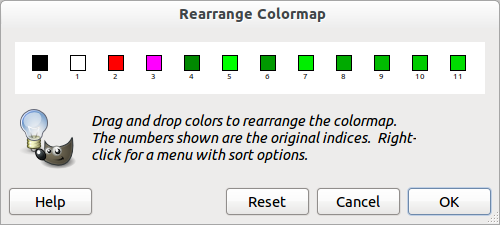
\includegraphics[scale=0.5]{images/gimp.png}
	\caption{Screenshot of the Rearrange Colormap dialog in Gimp 2.6.11}
	\label{gimpscreenshot}
	
\end{figure}
To manipulate the colormap, any slightly sophisticated image manipulation program should suffice. We used the free Software Gimp \cite{gimp}. It has a very comfortable command which allows the user to rearrange the colormap. This is shown in Figure~\ref{gimpscreenshot}.

\subsection{The Simulation Routines} % (fold)
\label{sub:The simulation Routines}

% subsection The simulation Routines (end)

\subsection{Output} % (fold)
\label{sub:Output}

% subsection Output (end)
\section{Simulation Results and Discussion}

\section{Summary and Outlook}

\section{References}
\bibliographystyle{plainnat}


\begingroup 
\renewcommand{\section}[2]{}%
\begin{thebibliography}{9}

	\bibitem{bbcnews}
		\url{http://www.bbc.co.uk/news/world-europe-16563562}, 9.12.2012
	\bibitem{multilevel}
	\emph{Modelling Situations of Evacuation
in a Multi-level Building} , 
Hans Hardmeier, Andrin Jenal, Beat Küng, Felix Thaler, Zurich, April 2012
	\bibitem{helbing}
		\emph{Simulating dynamical features of escape panic},
		Dirk Helbing, Ill\'es Farkas, Tam\'as Vicsek, Nature, 28. September 2000
	\bibitem{airplane}
		\emph{Pedestrian Dynamics Airplane Evacuation Simulation},
		Philipp Heer, Lukas Bühler, Zurich, May 2011
	\bibitem{gimp}
		\url{http://www.gimp.org/}, 9.12.2012
\end{thebibliography}
\endgroup



\end{document}  



 
